\section{Coquetel}
O Coquetel é um algoritmo de ordenação estável que traz a mesma ideia do Bolha, mas com um laço interno adicional. O primeiro laço, assim como no Bolha, itera da esquerda para a direita, empurrando os maiores elementos para o final do vetor, enquanto o segundo itera no outro sentido, empurrando os menores elementos para o início.

\lstinputlisting[language=C]{codigos/inf/2_coquetel.txt}

\subsection*{Corretude}
Ao final de uma iteração do laço externo, o menor e o maior elemento de $v[i..j]$ estarão nas posições $i$ e $j$, respectivamente. Dessa forma, ao final da primeira iteração, o menor elemento estará na posição $0$ e o maior, na posição $n - 1$; na segunda, o segundo menor, na posição $1$, e o segundo maior, na posição $n - 2$, e assim por diante. Esse processo garante que, quando $i \geq j$, o vetor estará ordenado; portanto, o algoritmo é correto.

\subsection*{Desempenho}
Embora as complexidades dos casos melhor, pior e médio continuem sendo, respectivamente, $\Theta(n)$, $\Theta(n^2)$ e \bigO{n^2}, o pior caso do Coquetel é menos frequente, pois ocorre apenas quando a entrada está em ordem decrescente.

\begin{figure}[H]
\Caption{\label{fig:coquetel_it}Coquetel aplicado ao vetor $[n, n-1, ..., 2, 1]$.}
\centering
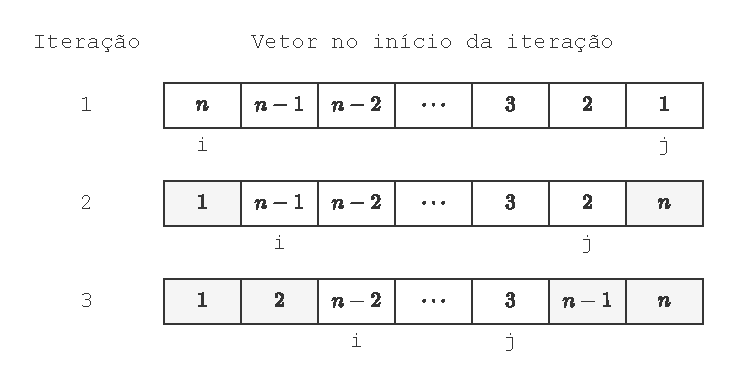
\includegraphics[scale=1.0]{figuras/pdf/coquetel.pdf}
\Fonte{Elaborado pelo autor.}
\end{figure}

Considere então que $T(n)$ é a quantidade total de iterações dos dois laços internos no pior caso. A figura \ref{fig:coquetel_it} ajuda a notar que a seguinte identidade é válida:

\[
T(n) = 
  \begin{cases}
      0,              & n < 2    \\
      T(n-2) + 2n - 3, & n \geq 2 
  \end{cases}
\]

Ao resolver a recorrência mostrada acima, pode-se observar que $T(n)$ é igual a soma \ref{eq:1}. Portanto, os algoritmos Bolha e Coquetel, em seus piores casos, executam exatamente a mesma quantidade de iterações.
